\documentclass[10pt]{article}
\usepackage{float}
\RequirePackage{eso-pic}
\usepackage{caption}
\captionsetup[table]{labelformat=empty}



\usepackage{geometry}
\geometry{
a4paper,
left=11mm,
right=14mm,
top=37mm,
bottom=14mm,
}



\usepackage{colortbl}
\usepackage{fontspec}
\setmainfont[Ligatures=TeX]{Calibri}



\newcommand\BackgroundPic{%
\put(0,0){%
\parbox[b][\paperheight]{\paperwidth}{%
\vfill
\centering
\includegraphics{MBIE_generic_background.pdf}%
\vfill
}}}



\begin{document}
\thispagestyle{empty}
\AddToShipoutPicture{\BackgroundPic}
\section*{Key Export Statistics\footnotemark - Cherries\footnotemark }
Published on April 11, 2016. \par
\small{\noindent{\textit{Monthly data from January 2000 to November 2015.}}}
\begin{table}[ht]
\centering
{\scriptsize
\begin{tabular}[t]{p{1.8cm}>{\hfill}p{1.4cm}>{\hfill}p{1.4cm}>{\hfill}p{1.6cm}>{\hfill}p{1.9cm}>{\hfill}p{2cm}>{\hfill}p{1.9cm}>{\hfill}p{1.5cm}}
 \textbf{Country} & \textbf{Yearly Qty} & \textbf{Yearly Value} & \textbf{Yearly Price} & \textbf{3Year CAGR(Qty)} & \textbf{3Year CAGR(Value)} & \textbf{3Year CAGR(Price)} & \textbf{Price Elasticity} \\
\hline
Taiwan & 1,163 & 20.3 & \$17.5 & 24.1\% & 28.7\% & 3.7\% & 6.5 \\  
China & 578 & 11.1 & \$19.2 & 355.2\% & 247.2\% & -23.7\% & -15.0 \\  
Thailand & 350 & 5.7 & \$16.2 & 21.5\% & 16.8\% & -3.9\% & -5.5 \\  
Vietnam & 242 & 4.0 & \$16.7 & 142.7\% & 115.9\% & -11\% & -12.9 \\  
Singapore & 160 & 2.6 & \$16.1 & 31.8\% & 26.9\% & -3.7\% & -8.7 \\  
South Korea & 140 & 2.1 & \$14.7 & 10.7\% & 6.7\% & -3.6\% & -2.9 \\  
Other & 289 & 5.1 & \$17.7 & 8\% & 7\% & -0.9\% & -8.9 \\  
Total & 2,922 & 50.9 & \$17.4 & 33.5\% & 34.5\% & 0.8\% & 42.6 \\  
\hline
\end{tabular}
}
\caption{\scriptsize Top 6 Cherries Markets for year ending November - 2015: Quantity('000 kg) Value(NZ\$Mill), Price and their last 3-Year Growth Rates}
\end{table}


\vspace{-0.7cm}



   \begin{figure}[H]
   \centering
    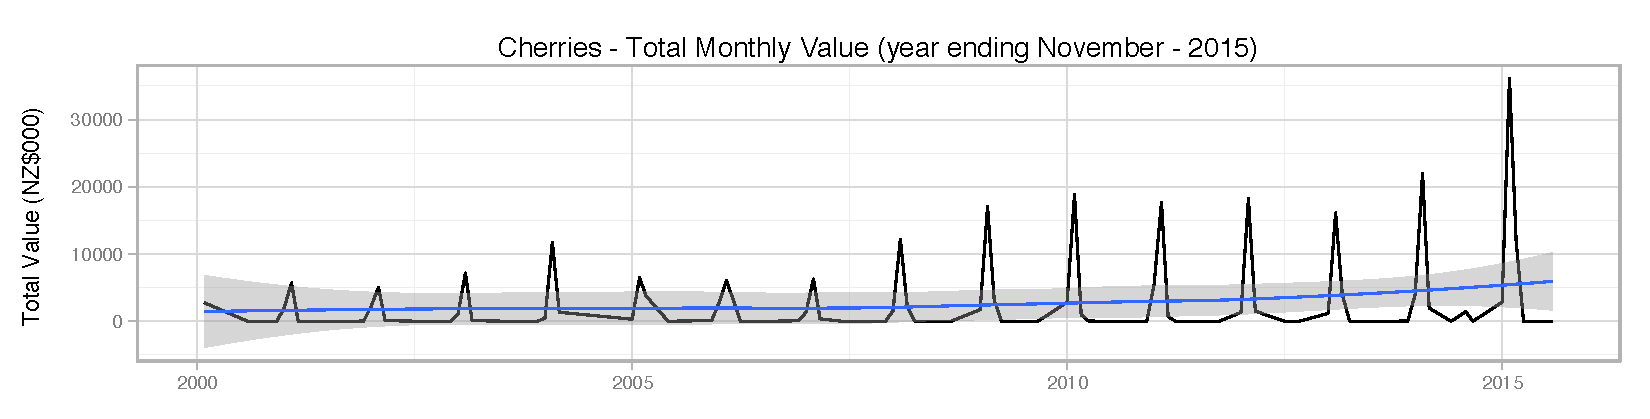
\includegraphics[scale=0.53]{../graphs/monthly_value/cherries_monthly_value.pdf} \
    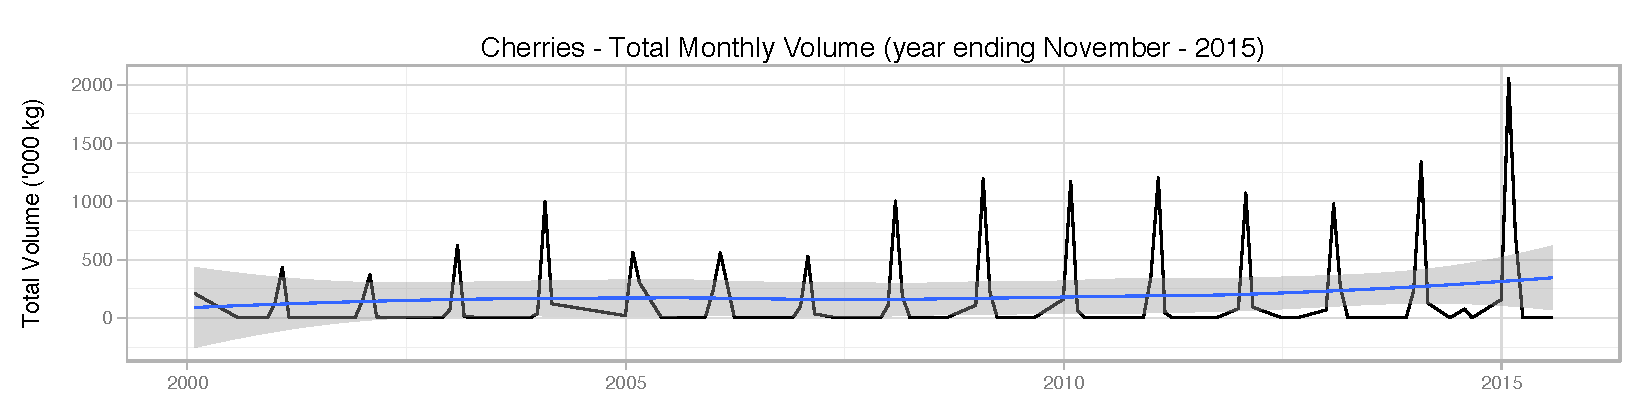
\includegraphics[scale=0.53]{../graphs/monthly_volume/cherries_monthly_volume.pdf} \
    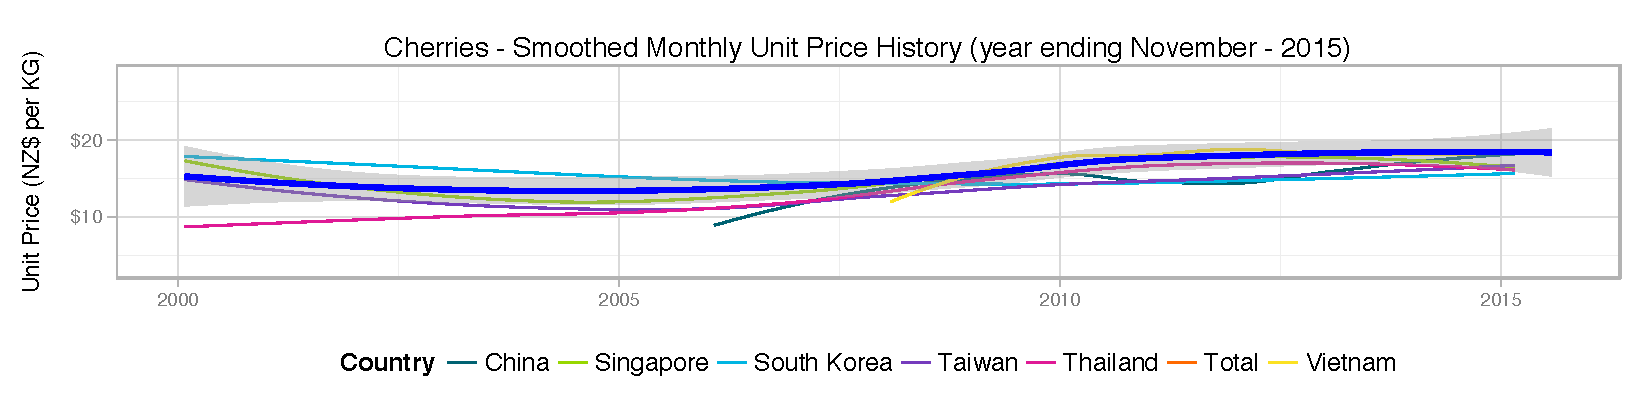
\includegraphics[scale=0.53]{../graphs/smoothed_price/cherries_smoothed_price.pdf} \
    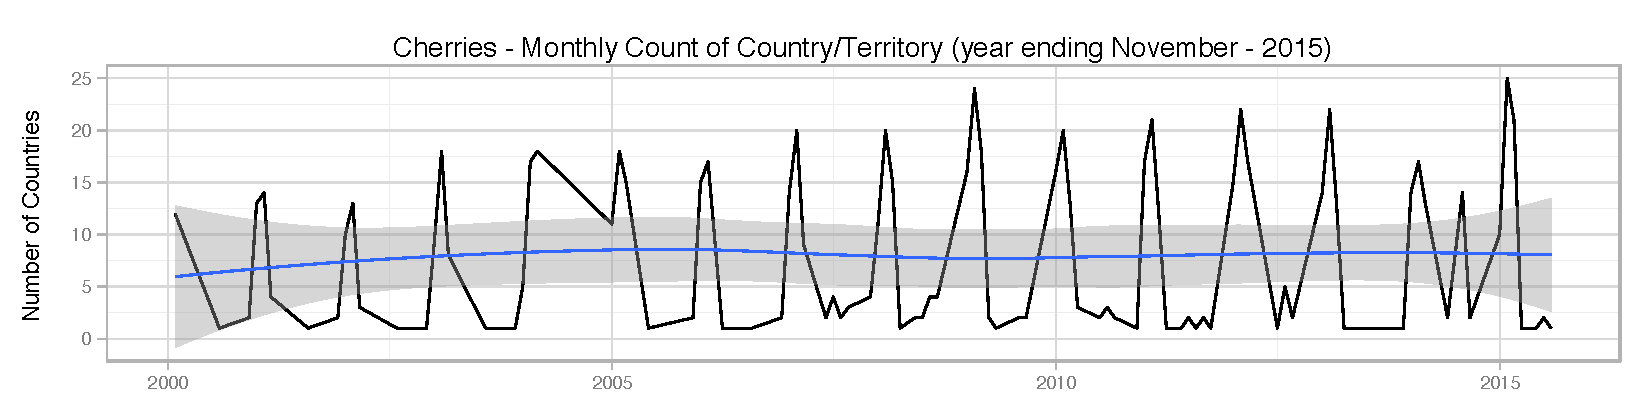
\includegraphics[scale=0.53]{../graphs/monthly_number_countries/cherries_monthly_count.pdf} \
    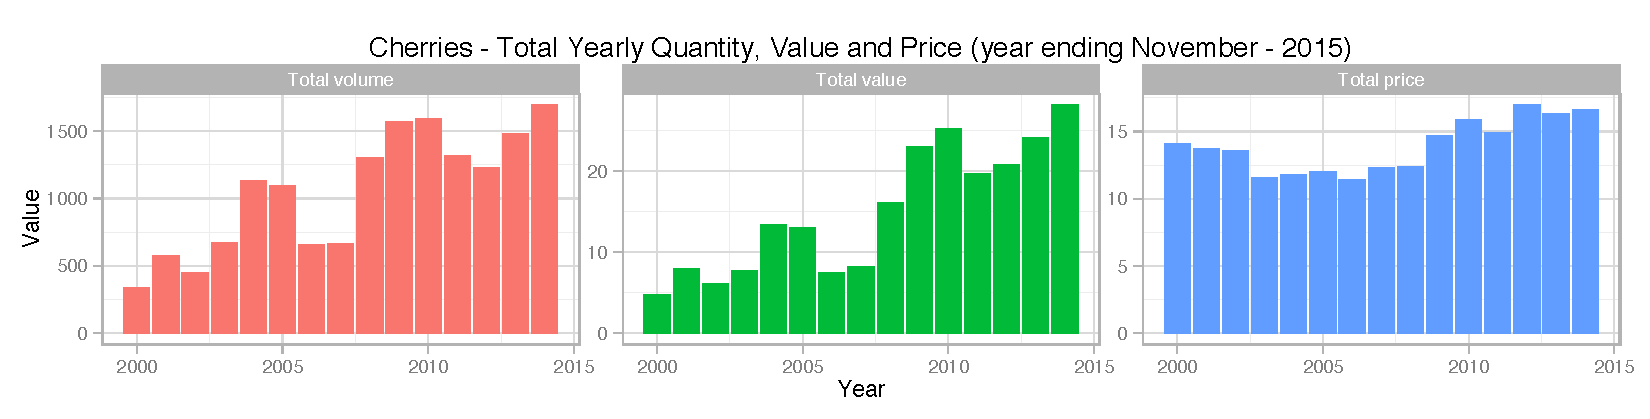
\includegraphics[scale=0.53]{../graphs/yearly_summary/cherries_yearly_summary.pdf} \
   \end{figure}



\footnotetext[1]{Source: Statistics New Zealand - Overseas Merchandise Trade}
\footnotetext[2]{Harmonised System Codes for Cherries starting with: 080920, 080921, 080929.}
\end{document}
